% MPC block diagram for the direct-prediction MPC supplementary figure (panel A).
% Style follows the R01 grant's fig_mpc.tex (rounded frame, model box inside the controller,
% plant box, feedback arrow), recoloured to the figure palette (MPC purple, cortex grey) and set
% in a sans font to match the JNeurosci panels. No parameter values (user 2026-10-09).
% Built by ctrl_mpc_direct_panels.m -> paper/images/supp_mpc/mpcd_0b_problem.pdf
\documentclass[border=1pt]{standalone}
\usepackage[scaled]{helvet}
\renewcommand\familydefault{\sfdefault}
\usepackage[T1]{fontenc}
\usepackage{sansmath}\sansmath
\newcommand{\Dl}{\mbox{\unsansmath$\Delta$}}
\usepackage{amsmath}
\usepackage{tikz}
\usetikzlibrary{arrows.meta,fit,backgrounds,positioning,calc}
\definecolor{mpc}{rgb}{0.45,0.20,0.60}
\definecolor{mpcl}{rgb}{0.96,0.93,0.98}
\definecolor{ink}{rgb}{0.38,0.38,0.38}
\begin{document}
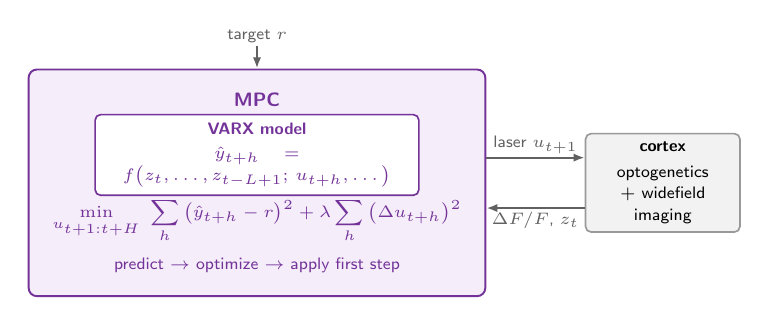
\begin{tikzpicture}[
  font=\fontsize{6.5}{7.8}\selectfont,
  mdl/.style ={rounded corners=2pt, draw=mpc, line width=0.6pt, align=center, fill=white,
               text=mpc, inner sep=3pt, text width=3.9cm},
  plt/.style ={rounded corners=2pt, draw=black!40, line width=0.6pt, align=center,
               fill=black!5, inner sep=3pt, text width=1.75cm, minimum height=1.25cm},
  frm/.style ={rounded corners=3pt, line width=0.7pt, draw=mpc, fill=mpcl, inner sep=5pt},
  sm/.style  ={font=\fontsize{6}{7.2}\selectfont, text=ink, inner sep=1pt},
  ar/.style  ={-{Latex[length=4pt,width=3pt]}, line width=0.8pt, draw=black!62}
]
\node[font=\bfseries\fontsize{7.5}{8.5}\selectfont, text=mpc] (mt) at (0,1.32) {MPC};
\node[mdl] (vx) at (0,0.62) {\textbf{VARX model}\\[1pt]
      $\hat y_{t+h} = f\big(z_{t},\dots,z_{t-L+1};\,u_{t+h},\dots\big)$};
\node[text=mpc, align=center] (cost) at (0,-0.22)
      {$\displaystyle\min_{u_{t+1:t+H}}\;\sum_{h}\big(\hat y_{t+h}-r\big)^2+\lambda\sum_{h}\big(\Dl u_{t+h}\big)^2$};
\node[text=mpc, font=\fontsize{6}{7.2}\selectfont] (vb) at (0,-0.78)
      {predict $\rightarrow$ optimize $\rightarrow$ apply first step};
\begin{scope}[on background layer]
  \node[frm, fit=(mt)(vx)(cost)(vb)] (MPC) {};
\end{scope}
\node[plt, right=1.25cm of MPC] (ctx) {\textbf{cortex}\\[2pt]{\fontsize{6}{7.2}\selectfont optogenetics\\$+$ widefield imaging}};
\node[sm, above=0.28cm of MPC.north] (ref) {target $r$};
\draw[ar] (ref) -- (MPC.north);
\draw[ar] ([yshift=0.32cm]MPC.east) -- node[sm, above] {laser $u_{t+1}$} ([yshift=0.32cm]ctx.west);
\draw[ar] ([yshift=-0.32cm]ctx.west) -- node[sm, below, align=center] {\Dl$F/F$, $z_t$} ([yshift=-0.32cm]MPC.east);
\end{tikzpicture}
\end{document}
